%-----------------begin---preamble-------------------
\documentclass[9pt]{beamer}
\usepackage{amsmath,amssymb,amsthm}
\usepackage{tikz,tkz-euclide}
\usepackage{enumerate}
\usepackage{cancel}


\usetikzlibrary{calc,patterns,angles,quotes}
\usetkzobj{all}

\usefonttheme{serif}
\usetheme{warsaw}%
\setbeamercovered{invisible}

\def\deg{^{\circ}}
\def\half{\frac{1}{2}}
\newcommand\heading[1]{\ \\\large{\textbf{#1}}}
\newcommand\ora[1]{\overrightarrow{#1}}


\newtheorem{notate}{Notation}
\newtheorem{cor}{Corollary}
% \newtheorem{examples}{Examples}
%------------------end---preamble--------------------
\title{Stellenbosch Camp 2018: Senior Geometry}
\subtitle{Lecture 4}
\author{Andrew McGregor}
\date{13 December 2018}

\begin{document}
	\frame{\titlepage}

	\begin{frame}
		\frametitle{Barycentric Coordinates}
		\only<1>{
		\begin{definition}[Barycentric Coordinates]
			Let $ABC$ be a triangle with an interior point $P$. The Barycentric coordinates of $P$ represent the relative ``weights'' that need to be placed at at the 3 vertices in order for $P$ to become the geometric centroid of the triangle. (I.e centre of gravity). 
		\end{definition}
		\begin{notate}[Barycentric Coordinates]
			Let $ABC$ be a triangle with an interior point $P$. Then the Barycentric coordinates of $P$ are written as $(\alpha,\beta,\gamma)$. Barycentric coordinates are also normalised so that $\alpha+\beta+\gamma=1$ (\textbf{This is important!}). 
		\end{notate}
		}
		\only<2>{
		\begin{examples}{Barycentric Coordinates}
			Let $ABC$ be a triangle. Here are the Barycentric coordinates of some well known points. For brevity, the normalisation for some of the points have been omitted.\\
			\begin{enumerate}
				\item {Triangle Vertices:  $A(1,0,0)$, $B(0,1,0)$, $C(0,0,1)$}
				\item {Centroid: $G\left(\frac{1}{3},\frac{1}{3},\frac{1}{3}\right)$}
				\item {Circumcentre: $O\left(a^{2} (S_a),  b^{2} (S_b), c^{2} (S_c)\right)$ }
				\item {Orthocentre: $H \left( S_c  S_b, S_a S_c,S_b S_a \right) $}
				\item {Incentre: \textbf{In Problem Set}}
				\item {Symmedian Point: $K(a^{2},b^{2},c^{2})$}
			\end{enumerate}
			Where $S_A=\frac{b^{2}+c^{2}-a^{2}}{2}$, $S_B=\frac{c^{2}+a^{2}-b^{2}}{2} $, and $S_C=\frac{a^{2}+b^{2}-c^{2}}{2}$
		\end{examples}
		}
		\only<3-5>{
			How do you find the barycentric coordinates of a point? \\
			\only<4-5>{If a point $P$ has Barycentric coordinates $(\alpha,\beta,\gamma)$, then the following diagram depicts the ratios that some segments are divided into.}
		}
		\only<6>{Lets do a problem.
		\begin{problem}
			Let $ABC$ be a triangle with an interior point $P$. Let $D$,$E$, and $F$ be the intersections of the lines $AP$, $BP$, and $CP$, with the lines $BC$,$CA$, and $AB$ respectively. Prove:
			\begin{flalign}
				\frac{PD}{DA}+\frac{PE}{EB}+\frac{PF}{FC}=1 \nonumber
			\end{flalign}
		\end{problem}}
		\only<7-9>{Usually with a problem like this, you would work out the ratios as ratios of areas of sub-triangles of $ABC$, and then add them together to show that the sum is 1. \uncover<8->{\textbf{Easy but laborious!}} \uncover<9>{So what about Barycentric coordinates? Do they make the problem easier?} }
		\only<10-12>{Using the result I showed you earlier you can immediately write down the following:\\
		\uncover<11->{Suppose $P$ has Barycentric coordinates $(\alpha,\beta,\gamma)$.}\uncover<12>{Then: $$\frac{PD}{DA}+\frac{PE}{EB}+\frac{PF}{FC}=\frac{\alpha}{\alpha+\beta+\gamma}+\frac{\beta}{\alpha+\beta+\gamma}+\frac{\gamma}{\alpha+\beta+\gamma}=1  $$} 
		}
		\only<13>{
		\begin{theorem}[Ceva's Theorem]
			Let $ABC$ be a triangle with points $D$, $E$, $F$ on sides $BC$, $CA$, and $AB$. The lines $AD$, $BE$, and $CF$ are concurrent if and only if
			\begin{flalign}
				\frac{AF}{FB} \cdot \frac{BD}{DC} \cdot \frac{CF}{FA}=1\nonumber
			\end{flalign}
		\end{theorem}
		}
		\only<14>{
		Suppose $P$ has Barycentric coordinates $(\alpha,\beta,\gamma)$
		\begin{flalign}
				\frac{AF}{FB} \cdot \frac{BD}{DC} \cdot \frac{CF}{FA}=\frac{\beta}{\alpha} \cdot \frac{\gamma}{\beta} \cdot \frac{\alpha}{\gamma}=1\nonumber
		\end{flalign}
		}
		\only<15>{
		Alternatively, another way to determine the barycentric coordinates is to use the ratio of areas of the opposite \textit{sub-triangle}.
		}
		\only<16>{
		\begin{definition}[Proportionality Theorem]
			Let $P(\alpha_1,\beta_1,\gamma_1)$, $Q(\alpha_2,\beta_2,\gamma_2)$ be 2 points in triangle $ABC$. If point $X$ that is on the line $PQ$, then 
			\begin{flalign}
				X=\frac{\ora{QX}\cdot(\alpha_1,\beta_1,\gamma_1)+\ora{XP}\cdot(\alpha_2,\beta_2,\gamma_2)}{PQ}
			\end{flalign}
			Coordinates are added component wise. Arrow overhead is to indicate directed edges.
		\end{definition}
		}
		\only<3>{
		\begin{figure}[!htb]
		\begin{center}
		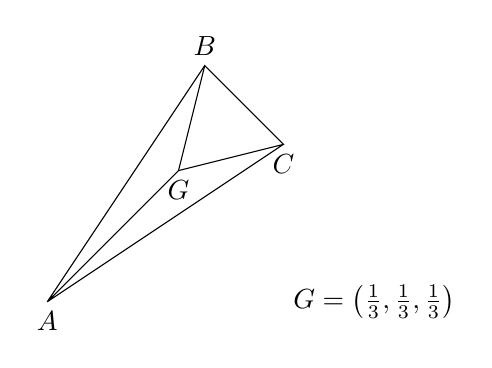
\begin{tikzpicture}[scale=1]
			\coordinate (A) at (-2,-1);
			\coordinate (B) at (0,2);
			\coordinate (C) at (1,1);
			\coordinate (G) at (barycentric cs:A=1 ,B=1 ,C=1);
			\draw[-] (A)--(B)--(C)--(G)--(A)--(C);
			\draw[-] (G)--(B);
			\node at (G) [below]{$G$};
			\node at (A) [below]{$A$};
			\node at (B) [above]{$B$};
			\node at (C) [below]{$C$};
			\node at (1,-1) [right]{$G=\left( \frac{1}{3},\frac{1}{3},\frac{1}{3} \right) $};
		\end{tikzpicture}
		\end{center}
		\end{figure}
		}
		\only<4-5>{
		\begin{figure}[!htb]
		\begin{center}
		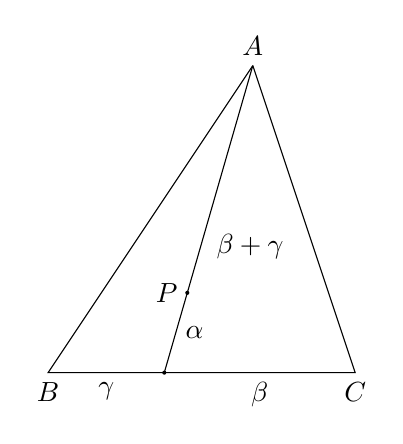
\begin{tikzpicture}[scale=1.3]
			\coordinate (B) at (-2,-1);
			\coordinate (A) at (0,2);
			\coordinate (C) at (1,-1);
			\coordinate (P) at (barycentric cs:A=1.3 ,B=2.3 ,C=1.4);
			\draw[-] (A)--(B)--(C)--(A);
			\node at (P) [left]{$P$};
			\node at (A) [above]{$A$};
			\node at (B) [below]{$B$};
			\node at (C) [below]{$C$};
			\tkzInterLL(A,P)(B,C)\tkzGetPoint{D};
			\fill[color=black!100] (P) circle (0.02) ;
			\fill[color=black!100] (D) circle (0.02) ;
			\draw[-] (A)--(P)--(D);
			\tkzLabelLine[below](B,D){$\gamma$};
			\tkzLabelLine[below](C,D){$\beta$};
			\tkzLabelLine[right](D,P){$\alpha$};
			\tkzLabelLine[below right,pos=0.3](P,A){$\beta+\gamma$};
		\end{tikzpicture}
		\end{center}
		\end{figure}
		}
		\only<6-14>{
		\begin{figure}[!htb]
		\begin{center}
		\begin{tikzpicture}[scale=1.2]
			\coordinate (B) at (-2,-1);
			\coordinate (A) at (0,2);
			\coordinate (C) at (1,-1);
			\coordinate (P) at (barycentric cs:A=1.3 ,B=2.3 ,C=1.4);
			\draw[-] (A)--(B)--(C)--(A);
			\node at (P) [below right=0.2 and 0]{$P$};
			\node at (A) [above]{$A$};
			\node at (B) [below]{$B$};
			\node at (C) [below]{$C$};
			\tkzInterLL(A,P)(B,C)\tkzGetPoint{D};
			\tkzInterLL(B,P)(A,C)\tkzGetPoint{E};
			\tkzInterLL(C,P)(A,B)\tkzGetPoint{F};
			\fill[color=black!100] (P) circle (0.02) ;
			\fill[color=black!100] (D) circle (0.02) ;
			\fill[color=black!100] (E) circle (0.02) ;
			\fill[color=black!100] (F) circle (0.02) ;
			\node at (D) [below]{$D$};
			\node at (E) [above right]{$E$};
			\node at (F) [above left]{$F$};
			\draw[-] (A)--(P)--(D);
			\draw[-] (B)--(P)--(E);
			\draw[-] (C)--(P)--(F);
			\only<12>{
			\tkzLabelLine[left](D,P){\small{$\alpha$}};
			\tkzLabelLine[right,pos=0.4](P,A){\small{$\beta+\gamma$}};
			\tkzLabelLine[below](E,P){\small{$\beta$}};
			\tkzLabelLine[left,pos=0.1](P,B){\small{$\alpha+\gamma$}};
			\tkzLabelLine[above](F,P){\small{$\gamma$}};
			\tkzLabelLine[right,pos=0.3](P,C){\small{$\alpha+\beta$}};
			}
			\only<12,14>{
			\tkzLabelLine[below](B,D){\small{$\gamma$}};
			\tkzLabelLine[below](C,D){\small{$\beta$}};
			\tkzLabelLine[above right](A,E){\small{$\gamma$}};
			\tkzLabelLine[above right](C,E){\small{$\alpha$}};
			\tkzLabelLine[above left](A,F){\small{$\beta$}};
			\tkzLabelLine[above left](B,F){\small{$\alpha$}};
			}
		\end{tikzpicture}
		\end{center}
		\end{figure}
		}
		\only<15>{
		\begin{figure}[!htb]
		\begin{center}
		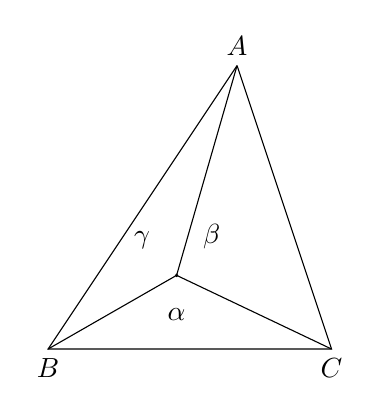
\begin{tikzpicture}[scale=1.2]
			\coordinate (B) at (-2,-1);
			\coordinate (A) at (0,2);
			\coordinate (C) at (1,-1);
			\coordinate (P) at (barycentric cs:A=1.3 ,B=2.3 ,C=1.4);
			\draw[-] (A)--(B)--(C)--(A);
			\node at (A) [above]{$A$};
			\node at (B) [below]{$B$};
			\node at (C) [below]{$C$};
			\fill[color=black!100] (P) circle (0.02) ;
			\draw[-] (A)--(P);
			\draw[-] (B)--(P);
			\draw[-] (C)--(P);
			\node at (P) [below=0.3]{$\alpha$};
			\node at (P) [above right=0.3]{$\beta$};
			\node at (P) [above left=0.3]{$\gamma$};
		\end{tikzpicture}
		\end{center}
		\end{figure}
		}
		\only<4-5>{\uncover<5>{\Huge{\textbf{You can claim this as well-known or common knowledge!}}}}
	\end{frame}
	\begin{frame}
		\frametitle{The Area Formula}
		\only<1>{
		\begin{theorem}
			Let $P(\alpha_1,\beta_1,\gamma_1)$, $Q(\alpha_2,\beta_2,\gamma_2)$ and $R(\alpha_3,\beta_3,\gamma_3)$ be points inside $\triangle ABC$. Then the area of $\triangle PQR$ is given by:
			\begin{flalign}
				|\triangle PQR|=\left|\begin{vmatrix}
				\alpha_1&\beta_1&\gamma_1\\
				\alpha_2&\beta_2&\gamma_2\\
				\alpha_3&\beta_3&\gamma_3
				\end{vmatrix}
				\right| |\triangle ABC|\nonumber
			\end{flalign}
			(Note that these coordinates are normalised.)
		\end{theorem}
		\begin{figure}[!htb]
		\centering
		\begin{tikzpicture}[scale=1.7]
			\tkzDefPoints{0/2/A,-1/0/B,1.5/0/C}
			\tkzDefBarycentricPoint(A=1,B=1,C=0.3)\tkzGetPoint{P}
			\tkzDefBarycentricPoint(A=0.4,B=1,C=0.7)\tkzGetPoint{Q}
			\tkzDefBarycentricPoint(A=0.1,B=0.6,C=1)\tkzGetPoint{R}
			\tkzDrawSegments(A,B B,C C,A P,Q Q,R R,P)
			\tkzLabelPoints[above](A,P)
			\tkzLabelPoints[below](B,C,Q)
			\tkzLabelPoints[right](R)
		\end{tikzpicture}
			
		\end{figure}
		}
		\only<2>{
		\begin{cor}[1]
			Let $P(\alpha_1,\beta_1,\gamma_1)$, $Q(\alpha_2,\beta_2,\gamma_2)$ and $R(\alpha_3,\beta_3,\gamma_3)$ be points inside $\triangle ABC$. Then $P$, $Q$ and $R$ are collinear if and only if
			\begin{flalign}
				\begin{vmatrix}
				\alpha_1&\beta_1&\gamma_1\\
				\alpha_2&\beta_2&\gamma_2\\
				\alpha_3&\beta_3&\gamma_3
				\end{vmatrix}=0\nonumber
			\end{flalign}
		\end{cor}
		}
		\only<3>{
		\begin{definition}[$3\times 3$ Determinant]
			\begin{flalign}
				\begin{vmatrix}
				x_1&y_1&z_1\\
				x_2&y_2&z_2\\
				x_3&y_3&z_3
				\end{vmatrix}=x_1 y_2 z_3+x_2 y_3 z_1+x_3 y_1 z_2-x_1 y_3 z_2-x_2 y_1 z_3-x_3 y_2 z_1\nonumber
			\end{flalign}
		\end{definition}
		}
		
	\end{frame}
	\begin{frame}
		\begin{problem}[Asiatic Pacific Maths Olympiad, 1989]
			Let $A_1, A_2, A_3$ be three points in the plane, and for convenience, let $A_4 = A_1$, $A_5 = A_2$. For $n = 1, 2$ and $3$, suppose that $B_n$ is the midpoint of $A_n A_{n+1}$ and suppose that $C_n$ is the midpoint of $A_n B_n$. Suppose that $A_n C_{n+1}$ and $B_n A_{n+2}$ meet at $D_n$ and that $A_n B_{n+1}$ and $C_n A_{n+2}$ meet at $E_n$. Calculate the ratio of the area of triangle $\triangle D_1 D_2 D_3$ to the area of triangle $\triangle E_1 E_2 E_3$.
		\end{problem}
			\begin{figure}[!htb]
			\begin{center}
			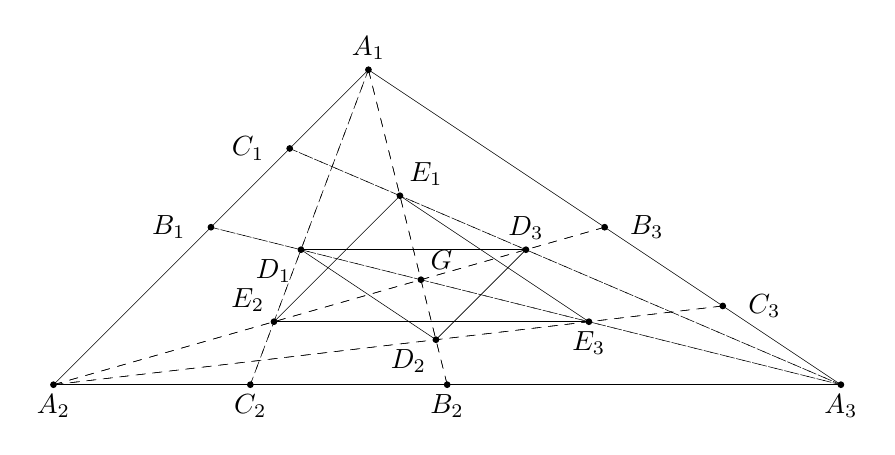
\begin{tikzpicture}[scale=2]
				% \useasboundingbox (-2,-2) rectangle  (2,2);
				\tkzDefPoint(0,2){A_1}
				\tkzDefPoint(-2,0){A_2}
				\tkzDefPoint(3,0){A_3}
				\tkzDefBarycentricPoint(A_1=1,A_2=1,A_3=1)\tkzGetPoint{G}
				\tkzDefBarycentricPoint(A_1=1,A_2=1)\tkzGetPoint{B_1}
				\tkzDefBarycentricPoint(A_2=1,A_3=1)\tkzGetPoint{B_2}
				\tkzDefBarycentricPoint(A_3=1,A_1=1)\tkzGetPoint{B_3}
				\tkzDefBarycentricPoint(A_1=1,B_1=1)\tkzGetPoint{C_1}
				\tkzDefBarycentricPoint(A_2=1,B_2=1)\tkzGetPoint{C_2}
				\tkzDefBarycentricPoint(A_3=1,B_3=1)\tkzGetPoint{C_3}
				\tkzInterLL(A_1,C_2)(B_1,A_3)\tkzGetPoint{D_1}
				\tkzInterLL(A_2,C_3)(B_2,A_1)\tkzGetPoint{D_2}
				\tkzInterLL(A_3,C_1)(B_3,A_2)\tkzGetPoint{D_3}
				\tkzInterLL(A_1,B_2)(C_1,A_3)\tkzGetPoint{E_1}
				\tkzInterLL(A_2,B_3)(C_2,A_1)\tkzGetPoint{E_2}
				\tkzInterLL(A_3,B_1)(C_3,A_2)\tkzGetPoint{E_3}
				\tkzDrawSegments(A_1,A_2 A_2,A_3 A_3,A_1)
				\tkzDrawSegments[dashed](A_1,C_2 A_2,C_3 A_3,C_1 A_1,B_2 A_2,B_3 A_3,B_1)
				\tkzDrawSegments[dashed](B_1,A_3 B_2,A_1 B_3,A_2 C_1,A_3 C_2,A_1 C_3,A_2)
				\tkzDrawSegments(D_1,D_2 D_2,D_3 D_3,D_1)
				\tkzDrawSegments(E_1,E_2 E_2,E_3 E_3,E_1)
				\tkzDrawPoints[fill=black](A_1,A_2,A_3,B_1,B_2,B_3,C_1,C_2,C_3,D_1,D_2,D_3,E_1,E_2,E_3,G)
				\tkzLabelPoints[above](A_1,D_3)
				\tkzLabelPoints[right=0.2](B_3,C_3)
				\tkzLabelPoints[below](A_2,A_3,B_2,C_2,E_3)
				\tkzLabelPoints[left=0.2](B_1,C_1)
				\tkzLabelPoints[above left](E_2)
				\tkzLabelPoints[above right](E_1,G)
				\tkzLabelPoints[below left](D_2,D_1)
				\end{tikzpicture}
			\end{center}		
			\end{figure}
	\end{frame}


\end{document}